\documentclass[a4paper,11pt]{article}
\usepackage[utf8]{inputenc}
\usepackage[T1]{fontenc}
\usepackage[french]{babel}
\usepackage{amsmath}
\usepackage[top=2cm, bottom=2cm, left=2.1cm, right=2.1cm]{geometry}
\usepackage{xcolor}
\usepackage{graphicx}
\usepackage{booktabs}
\usepackage{tabularx}
\usepackage{enumitem}
\usepackage{listings}
\usepackage{titlesec}
\usepackage[most]{tcolorbox}
\usepackage{tikz}
\usetikzlibrary{arrows.meta, positioning, shapes.geometric, fit, backgrounds, calc}
\usepackage{hyperref}
\hypersetup{colorlinks=true, linkcolor=primary, urlcolor=primary, citecolor=primary}

% ---- palette ----
\definecolor{primary}{HTML}{1A237E}
\definecolor{accent}{HTML}{00695C}
\definecolor{success}{HTML}{2E7D32}
\definecolor{warning}{HTML}{C62828}
\definecolor{codebg}{HTML}{F7F8FA}
\definecolor{kw}{HTML}{7B1FA2}
\definecolor{cm}{HTML}{8D9199}
\definecolor{str}{HTML}{2E7D32}
\definecolor{layP}{HTML}{E8EAF6}
\definecolor{layD}{HTML}{FFF3E0}
\definecolor{layC}{HTML}{E0F2F1}

% ---- styles code ----
\lstdefinestyle{py}{language=Python, backgroundcolor=\color{codebg},
  basicstyle=\ttfamily\scriptsize, keywordstyle=\color{kw}\bfseries,
  commentstyle=\color{cm}\itshape, stringstyle=\color{str},
  breaklines=true, frame=leftline, framerule=1.5pt, rulecolor=\color{accent},
  framesep=6pt, showstringspaces=false, columns=fullflexible}
\lstdefinestyle{cpp}{language=C++, backgroundcolor=\color{codebg},
  basicstyle=\ttfamily\scriptsize, keywordstyle=\color{primary}\bfseries,
  commentstyle=\color{cm}\itshape, stringstyle=\color{str},
  breaklines=true, frame=leftline, framerule=1.5pt, rulecolor=\color{primary},
  framesep=6pt, showstringspaces=false, columns=fullflexible}

\titleformat{\section}{\large\bfseries\color{primary}}{\thesection.}{0.6em}{}
\titlespacing*{\section}{0pt}{11pt}{4pt}
\titleformat{\subsection}{\bfseries\color{accent}}{\thesubsection.}{0.5em}{}
\titlespacing*{\subsection}{0pt}{6pt}{2pt}
\setlength{\parindent}{0pt}
\setlength{\parskip}{3.5pt}
\newcommand{\code}[1]{\texttt{\small #1}}

\newtcolorbox{note}[1][Résultat]{colback=success!6, colframe=success, fonttitle=\bfseries,
  title=#1, boxrule=0.6pt, left=6pt, right=6pt, top=3pt, bottom=3pt}
\newtcolorbox{contrib}[1][Ma contribution]{colback=primary!5, colframe=primary, fonttitle=\bfseries,
  title=#1, boxrule=0.6pt, left=6pt, right=6pt, top=3pt, bottom=3pt}

\title{\textbf{Système de sécurité coopérative V2V}\\[5pt]
  {\large\mdseries De la perception par IA à l'alerte coopérative (messages CAM et DENM)}}
\author{Douae Sebti \\[2pt] {\small Tuteur académique : Samuel Dupont}}
\date{Rapport hebdomadaire --- semaine du 7 au 13 juillet 2026}

\begin{document}
\maketitle
\vspace{-2pt}
\begin{center}\rule{0.96\textwidth}{0.4pt}\end{center}
\vspace{3pt}

\begin{contrib}[En une phrase]
Ma voiture détecte un obstacle (caméra RGB-D + réseau de neurones YOLO), décide un freinage, et
diffuse une alerte normalisée ETSI (message \textbf{DENM}) que le véhicule voisin reçoit et
affiche --- le tout en parallèle des messages de présence (\textbf{CAM}) enrichis de la position,
du cap et de la vitesse.
\end{contrib}

\begin{contrib}[Ma contribution]
Ce travail --- perception par IA (YOLO + profondeur), enrichissement des messages CAM et
implémentation des messages DENM, puis intégration et démonstration --- constitue ma contribution
au projet ProtoVA.
\end{contrib}

\tableofcontents
\vspace{4pt}
\begin{center}\rule{0.96\textwidth}{0.4pt}\end{center}

% ======================= 1. CONTEXTE =======================
\section{Contexte : les systèmes coopératifs (C-ITS)}
Un véhicule ne « voit » que ce que ses capteurs perçoivent. Les \textbf{systèmes coopératifs}
(C-ITS) lèvent cette limite : les véhicules s'échangent des messages pour se signaler, anticiper
un freinage, prévenir d'un obstacle. L'ETSI normalise deux messages complémentaires que
j'exploite ici :
\begin{itemize}[leftmargin=1.5em, itemsep=1pt]
  \item \textbf{CAM} (\emph{Cooperative Awareness Message}, ETSI EN 302~637-2) --- périodique :
        « je suis là, telle position, tel cap, telle vitesse ».
  \item \textbf{DENM} (\emph{Decentralized Environmental Notification Message}, ETSI EN 302~637-3)
        --- événementiel : « attention, danger à cet endroit ».
\end{itemize}
\textbf{Objectif de la semaine :} qu'un obstacle détecté déclenche \emph{automatiquement} un
DENM, reçu et affiché par un autre véhicule --- soit une boucle \emph{percevoir $\to$ alerter
$\to$ réagir} complète.

% ======================= 2. ARCHITECTURE =======================
\section{Vue d'ensemble : une architecture en trois couches}
J'ai structuré le système en trois couches (figure~\ref{fig:archi}) : la
\textcolor{primary}{\textbf{perception}} (voir et décider), la \textcolor{warning}{\textbf{décision}}
(freiner et déclencher l'alerte), et la \textcolor{accent}{\textbf{communication}} (la pile ETSI
C-ITS qui diffuse le message sur le réseau).

\begin{figure}[h]\centering
\resizebox{\textwidth}{!}{%
\begin{tikzpicture}[font=\footnotesize,
  L/.style={draw, rounded corners=3pt, align=center, minimum height=9mm, inner sep=4pt, thick},
  p/.style={L, fill=layP, draw=primary}, d/.style={L, fill=layD, draw=warning},
  c/.style={L, fill=layC, draw=accent},
  fl/.style={-{Latex[length=2.4mm]}, very thick},
  st/.style={draw=accent, fill=layC, minimum width=52mm, minimum height=6.5mm, inner sep=2pt, align=center}]

  % --- couche perception ---
  \node[p] (cam)  {Caméra RGB-D\\ \scriptsize couleur + profondeur};
  \node[p, right=6mm of cam]  (yolo) {YOLOv8\\ \scriptsize détection d'objets};
  \node[p, right=6mm of yolo] (dist) {Profondeur\\ \scriptsize distance de l'obstacle};
  % --- couche decision ---
  \node[d, right=8mm of dist] (dec) {Décision\\ \scriptsize \code{/obstacle/brake}};
  % --- couche communication (pile ETSI) a droite ---
  \node[st, right=10mm of dec] (fac) {\textbf{Facilities} : CAM / \textbf{DENM}};
  \node[st, below=1.2mm of fac] (btp) {BTP (transport)};
  \node[st, below=1.2mm of btp] (gn)  {GeoNetworking};
  \node[st, below=1.2mm of gn]  (acc) {Accès WiFi (multicast)};

  % fleches perception -> decision
  \draw[fl, primary] (cam)  -- (yolo);
  \draw[fl, primary] (yolo) -- (dist);
  \draw[fl, warning] (dist) -- (dec);
  \draw[fl, warning] (dec)  -- (fac.west);
  % pile descendante
  \draw[fl, accent] (fac) -- (btp);
  \draw[fl, accent] (btp) -- (gn);
  \draw[fl, accent] (gn)  -- (acc);

  % vehicule B (recepteur) sous la pile
  \node[c, below=9mm of acc] (rx) {\textbf{Véhicule B} : réception $\to$ décodage $\to$
    \textbf{\textcolor{warning}{ALERTE}}};
  \draw[fl, accent] (acc) -- (rx) node[midway, right=1mm]{\scriptsize DENM (WiFi)};

  % cadres de couches
  \begin{scope}[on background layer]
    \node[draw=primary!40, dashed, rounded corners, inner sep=5mm, fit=(cam)(yolo)(dist),
      label={[primary, font=\bfseries]above:PERCEPTION}] {};
    \node[draw=warning!50, dashed, rounded corners, inner sep=3mm, fit=(dec),
      label={[warning, font=\bfseries]above:DÉCISION}] {};
    \node[draw=accent!50, dashed, rounded corners, inner sep=3mm, fit=(fac)(acc),
      label={[accent, font=\bfseries]above:COMMUNICATION (pile ETSI C-ITS)}] {};
  \end{scope}
\end{tikzpicture}}
\caption{Architecture en trois couches. La perception (bleu) alimente la décision (rouge) qui
déclenche l'émission d'un message via la pile normalisée ETSI (vert), reçu par le véhicule voisin.}
\label{fig:archi}
\end{figure}

% ======================= 3. PERCEPTION =======================
\section{Couche perception : voir et mesurer}
La caméra \textbf{Orbbec Femto Bolt} fournit une image couleur (1280$\times$720, $\sim$14~img/s)
et une image de \textbf{profondeur}. \textbf{YOLOv8} détecte les objets ; la profondeur donne
leur distance. Le point délicat est l'\emph{estimation de distance} : une boîte englobante
contient aussi de l'arrière-plan, et la médiane fausse le résultat pour un objet proche. Je
retiens donc le \textbf{point le plus proche} de l'objet (percentile bas), robuste au bruit :

\begin{lstlisting}[style=py]
# Distance a l'obstacle = sa surface AVANT (percentile 20), pas la mediane
v = depth_m[region_centrale]            # profondeurs dans la boite
v = v[(v > 0.15) & (v < 20.0)]          # ignore les pixels invalides (0)
distance = np.percentile(v, 20)         # le point le plus proche = ce qui compte
\end{lstlisting}

La décision de freinage est ensuite \emph{indépendante de la classe} : tout obstacle proche
compte, un objet loin est ignoré.

\begin{lstlisting}[style=py]
proche = (distance is not None and distance < seuil_freinage)
if proche:                              # n'importe quel obstacle proche
    brake = True                        # -> /obstacle/brake -> declenche le DENM
\end{lstlisting}

\begin{figure}[h]\centering
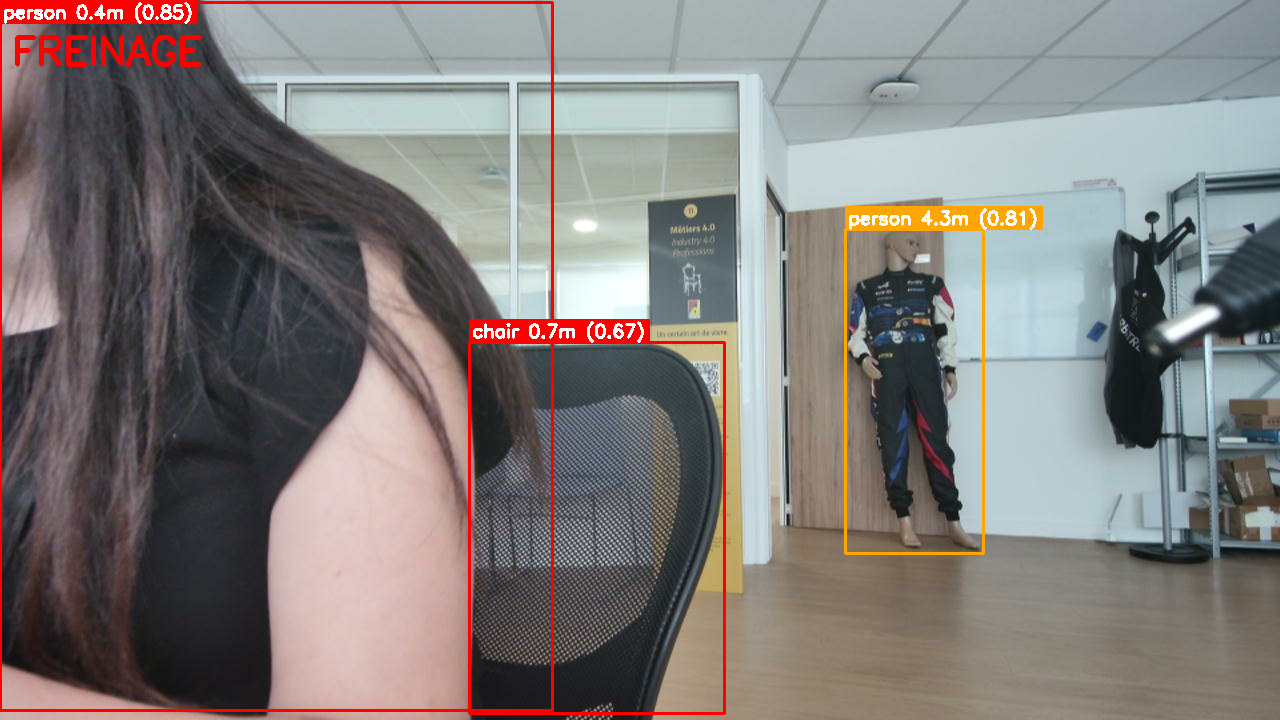
\includegraphics[width=0.78\textwidth]{img_detection_yolo.png}
\caption{Détection en temps réel sur la caméra du véhicule : classe, distance et confiance sur
chaque objet ; code couleur \textcolor{warning}{rouge = obstacle proche (freinage)},
vert/orange = objet éloigné. « FREINAGE » s'affiche quand un obstacle est trop proche.}
\end{figure}

\begin{contrib}
Deux verrous levés : (i) l'\textbf{alignement profondeur-sur-couleur} (les capteurs ont des
champs différents, $f\!\approx\!747$~px en couleur contre $505$~px en profondeur ; sans recalage,
les distances sont fausses) ; (ii) le passage de la médiane au \textbf{percentile du plus proche},
qui corrige les distances aberrantes des objets très proches.
\end{contrib}

% ======================= 4. CAM =======================
\section{Couche communication (1) : le CAM enrichi}
Le CAM annonce en continu l'état du véhicule. Je l'ai \textbf{enrichi} du \textbf{cap} et de la
\textbf{vitesse} réels (auparavant à zéro), calculés depuis l'odométrie et propagés jusqu'au
message émis :

\begin{lstlisting}[style=py]
# Cap depuis l'orientation (lacet du quaternion), vitesse depuis le twist
yaw     = atan2(2*(qw*qz + qx*qy), 1 - 2*(qy*qy + qz*qz))
heading = degrees(yaw) % 360.0          # cap Nord vrai [0, 360[
speed   = hypot(vx, vy)                  # vitesse (m/s)
publish([lat, lon, heading, speed])      # -> rempli dans le CAM emis
\end{lstlisting}

\begin{figure}[h]\centering
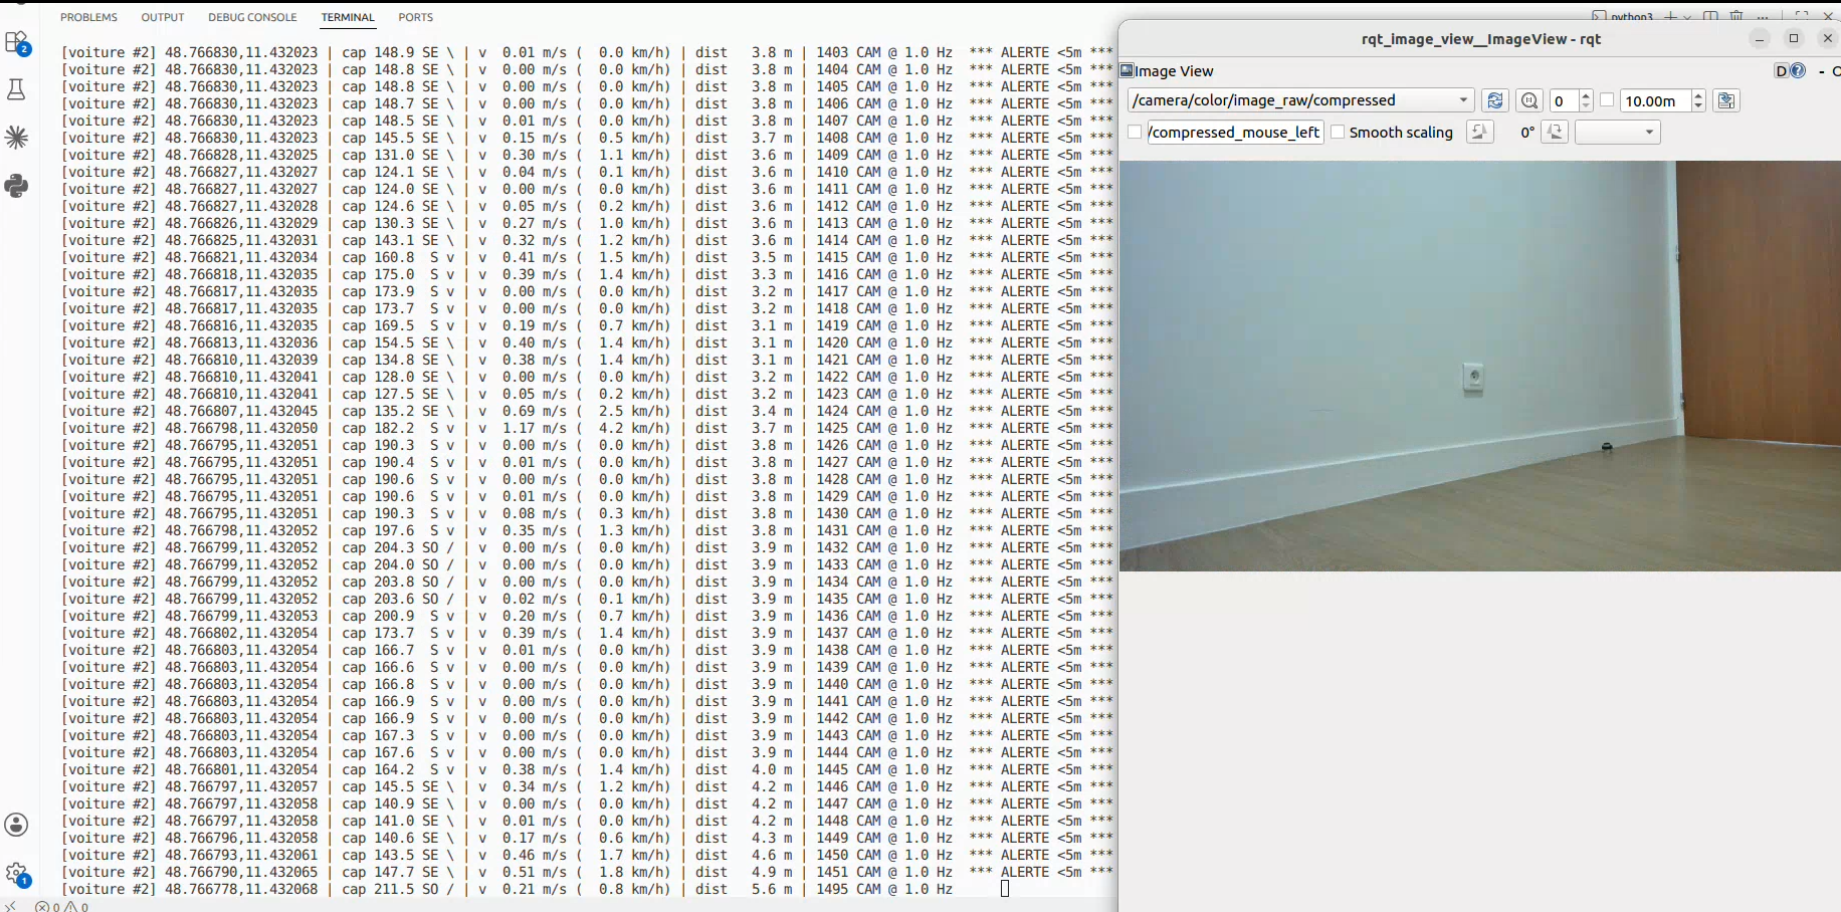
\includegraphics[width=0.93\textwidth]{img_cam_monitor.png}
\caption{Réception des CAM en direct (moniteur développé) : position, cap (boussole), vitesse
(m/s et km/h) et distance du véhicule voisin, à $\sim$1~Hz, avec le flux vidéo de la caméra.}
\end{figure}

% ======================= 5. DENM =======================
\section{Couche communication (2) : le DENM (contribution centrale)}
L'outil \code{socktap} ne savait émettre que des CAM. J'ai développé une \textbf{application
DENM} qui construit un message d'événement ETSI conforme et le diffuse sur commande :

\begin{lstlisting}[style=cpp]
// DENM : message d'evenement ETSI. Ou est le danger + de quel type.
copy(position, mgmt.eventPosition);          // position de l'evenement
sit->eventType.causeCode    = 99;            // dangerousSituation
sit->eventType.subCauseCode = 2;             // emergencyElectronicBrakeEngaged
request.transport_type = TransportType::SHB; // diffusion 1 saut (broadcast)
send(request, denm);                         // -> les vehicules voisins
\end{lstlisting}

L'émission est déclenchée par ROS lorsque \code{/obstacle/brake} passe à vrai ; à la réception,
le DENM est décodé et affiché comme une alerte. La figure~\ref{fig:seq} résume l'échange.

\begin{figure}[h]\centering
\resizebox{0.92\textwidth}{!}{%
\begin{tikzpicture}[font=\footnotesize,
  life/.style={draw, thick, dashed, gray}, ev/.style={draw, rounded corners=2pt, align=center, inner sep=3pt}]
  % lignes de vie
  \node[ev, fill=layP, draw=primary] (A) {\textbf{Véhicule A}\\ \scriptsize perception};
  \node[ev, fill=layC, draw=accent, right=75mm of A] (B) {\textbf{Véhicule B}\\ \scriptsize récepteur};
  \draw[life] (A) -- ++(0,-4.6);
  \draw[life] (B) -- ++(0,-4.6);
  \coordinate (A0) at ($(A.south)+(0,-0.5)$);
  \coordinate (B0) at ($(B.south)+(0,-0.5)$);
  % CAM continus (bidirectionnels)
  \draw[-{Latex}, accent] ($(A0)$) -- ++(75mm,0) node[midway, above]{\scriptsize CAM (position, cap, vitesse) $\sim$1~Hz};
  \draw[{Latex}-, accent] ($(A0)+(0,-0.5)$) -- ++(75mm,0) node[midway, below]{\scriptsize CAM};
  % detection sur A
  \node[ev, fill=layD, draw=warning] (det) at ($(A0)+(0,-1.7)$) {\scriptsize YOLO : piéton à $<2$~m $\Rightarrow$ freinage};
  % DENM A->B
  \draw[-{Latex}, very thick, warning] ($(A0)+(0,-2.6)$) -- ++(75mm,0)
    node[midway, above]{\scriptsize \textbf{DENM} (cause 99/2, position)};
  % alerte sur B
  \node[ev, fill=warning!12, draw=warning] (al) at ($(B0)+(0,-3.3)$) {\scriptsize \textbf{ALERTE} affichée};
\end{tikzpicture}}
\caption{Séquence d'échange : les CAM circulent en continu ; à la détection d'un obstacle, le
véhicule A émet un DENM que B reçoit et transforme en alerte.}
\label{fig:seq}
\end{figure}

\begin{figure}[h]\centering
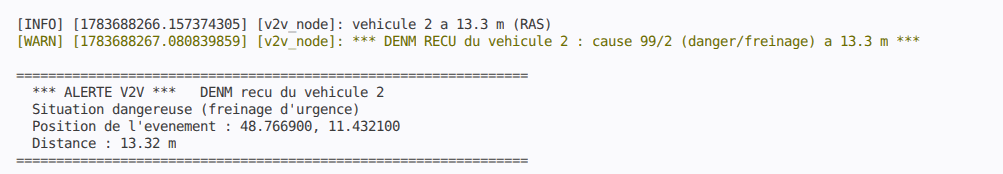
\includegraphics[width=0.82\textwidth]{denm_msg2.png}
\caption{Côté récepteur : le DENM émis par le véhicule qui freine est reçu, décodé (émetteur,
cause « situation dangereuse / freinage d'urgence », position, distance) et affiché comme alerte.}
\end{figure}

\textbf{CAM et DENM sont simultanés} : un même processus gère les deux (option \code{-a ca den}).
Le CAM circule en permanence ; le DENM ne part qu'en cas d'événement.

% ======================= 6. RESULTATS =======================
\section{Résultats}
\begin{center}\small
\begin{tabularx}{\textwidth}{@{}l l X@{}}
\toprule
\textbf{Grandeur} & \textbf{Mesure} & \textbf{Commentaire} \\
\midrule
Détection (personne) & confiance 0,8--0,94 & YOLOv8, temps réel \\
Distance mesurée & 0,4 m à 4,3 m & différenciée après recalage profondeur \\
CAM & $\sim$1 Hz, $\sim$99 octets & conforme EN 302 637-2 \\
DENM & cause 99 / sous-cause 2 & \emph{dangerousSituation / freinage d'urgence} \\
Réception & cause + position + distance & décodé et affiché sur le 2\textsuperscript{e} véhicule \\
Lien & WiFi multicast, sans 802.11p & \emph{Single Hop Broadcast} \\
\bottomrule
\end{tabularx}
\end{center}

\begin{note}[Validé en conditions réelles]
Chaîne complète démontrée : \emph{perception $\to$ freinage $\to$ DENM émis $\to$ DENM reçu
$\to$ alerte}, en parallèle des CAM, entre deux calculateurs sur des domaines ROS séparés (la
communication passe donc bien par le V2V, pas par le bus interne).
\end{note}

% ======================= 7. DIFFICULTES =======================
\section{Difficultés techniques et solutions}
\begin{itemize}[leftmargin=1.5em, itemsep=1pt]
  \item \textbf{Distances erronées} $\to$ activation de l'alignement profondeur-sur-couleur.
  \item \textbf{Objet proche mal mesuré} (boîte englobant l'arrière-plan) $\to$ distance prise au
        point le plus proche (percentile), pas à la médiane.
  \item \textbf{Messages rejetés} (\emph{decap unsuccessful}) $\to$ émetteur et récepteur doivent
        partager la même configuration de sécurité.
  \item \textbf{Latence caméra sur WiFi} ($\sim$100--250~ms) $\to$ justifie d'embarquer à terme la
        décision sur le véhicule.
\end{itemize}

% ======================= 8. LIMITES =======================
\section{Limites et perspectives (semaine prochaine)}
\textbf{Limites.} La détection tourne sur le PC (flux caméra du véhicule), pas encore embarquée ;
YOLO ne reconnaît que ses classes apprises ; démonstration sur WiFi, messages non signés.

\textbf{Perspectives.}
\begin{enumerate}[leftmargin=1.5em, itemsep=1pt]
  \item \textbf{embarquer YOLO} sur la Jetson (optimisé TensorRT) $\to$ détection et freinage
        autonomes à bord, sans latence réseau ;
  \item \textbf{fusion LiDAR + caméra} : le LiDAR voit la géométrie (tout obstacle), YOLO donne le
        sens (piéton) ;
  \item \textbf{réaction physique} : buzzer / LED puis freinage d'urgence automatique (AEB) ;
  \item \textbf{passage 5G} et \textbf{messages signés} (certificats, sécurité C-ITS complète).
\end{enumerate}

% ======================= 9. CONCLUSION =======================
\section{Conclusion}
J'ai obtenu une boucle de sécurité coopérative complète : \emph{percevoir} (IA + profondeur),
\emph{décider} (freinage), \emph{alerter} (DENM ETSI), \emph{recevoir et afficher}. Les messages
CAM et DENM, conformes aux normes, circulent en parallèle sur un WiFi ordinaire. La suite visera
l'embarquement de la perception et la réaction physique jusqu'au freinage automatique.

\vspace{4pt}\hrule
{\footnotesize\textbf{Références normatives.} ETSI EN 302~637-2 (CAM) ; EN 302~637-3 (DENM) ;
EN 302~636-4-1 (GeoNetworking) ; EN 302~636-5-1 (BTP) ; TS 102~894-2 (dictionnaire de données) ;
pile Vanetza (implémentation open-source C-ITS).}

\end{document}
